\documentclass[12pt,twoside]{report} % Two side
% \documentclass[12pt]{report} % One side
\usepackage[utf8]{inputenc}
\usepackage[dutch]{babel}

\usepackage{titling}

% Todo notes
\usepackage{todonotes}

% Setup page margins
\usepackage[a4paper,width=165mm,top=25mm,bottom=25mm,bindingoffset=10mm]{geometry}
% custom commands
% Setup header & footer
\usepackage{fancyhdr}
\pagestyle{fancy}
\fancyhf{}
\setlength{\headheight}{15pt}
% \fancyhead[RO,LE]{\leftmark} % Two side
% \fancyfoot[RO,LE]{\thepage}
% \fancyfoot[CO,CE]{Proposal}

\fancyhead[L]{\MakeUppercase{\leftmark}}
% \fancyhead[C,C]{\leftmark} % One side
\fancyfoot[R,R]{\thepage}
\fancyfoot[C,C]{Plan van Aanpak}

% No header & footer on empty pages
\usepackage{emptypage}

% Monkeypatch chapters to use the 'fancy' style
\usepackage{etoolbox}
\patchcmd{\chapter}{\thispagestyle{plain}}{\thispagestyle{fancy}}{}{}

% Configure list spacing
\usepackage{enumitem}
\setlist{nosep} % or \setlist{noitemsep} to leave space around whole list

% Gantt charts
\usepackage{pgfgantt}

% Tables
\usepackage{tabularx}
\usepackage{makecell}
% Plots
\usepackage{pgfplots}
\pgfplotsset{width=10cm,compat=1.9}

% Captions
\usepackage{caption}
\captionsetup{labelfont=bf, font=footnotesize, hypcap=true, skip=5pt, width=0.9\textwidth}
% Rotating figures
\usepackage{rotating}

% Load glossary
% \usepackage{glossaries}
\usepackage[nonumberlist]{glossaries}
\makenoidxglossaries

\newglossaryentry{CMS}
{
	name={Content management systeem},
	description={Een contentmanagementsysteem is een softwaretoepassing,
			meestal een webapplicatie, die het mogelijk maakt dat mensen eenvoudig, zonder veel technische kennis,
			documenten en gegevens op internet kunnen publiceren (contentmanagement).
			Als afkorting wordt ook wel CMS gebruikt},
	first={content management systeem (CMS)},
	text={CMS}
}
\newglossaryentry{GUI}
{
	name={Graphical user interface},
	description={Een graphical user interface, is een manier van interacteren met een computer waarbij grafische beelden, widgets en tekst gebruikt worden},
	first={graphical user interface (GUI)},
	text={GUI}
}
\newglossaryentry{SDLC}
{
	name={Software development life cycle},
	description={de software development life cycle (SDLC) is een process matige manier van werken met als doel goede kwaliteit software te produceren met lage kosten in een korte tijd.
    De SDLC bestaat uit 5 fases: \textit{Requirements analysis}, \textit{Design}, \textit{Implementation}, \textit{Testing}, en \textit{Evolution} \Parencite{SDLC}},
	first={software development life cycle (SDLC)},
	text={SDLC}
}
\newglossaryentry{SEO}{
    name={Search engine optimization},
    description = {Search Engine Optimisation, zijn alle processen en verbeteringen die als doen hebben een website hoger in Google te laten verschijnen},
    first = {search engine optimization (SEO)},
    text = {SEO}
}
\newglossaryentry{UserJourneys}{
    name={User journeys},
    description = {User journeys zijn de verschillende acties die een gebruiker moet uit voeren (Meestal via een interface) om een eind resultaat te bereiken},
    first = {user journeys},
    text = {user journeys}
}


% Censoring
\usepackage{censor} \StopCensoring

% Citations
% \usepackage{biblatex-apa}
\usepackage{csquotes}
\usepackage[backend=biber, style=apa, urldate=long]{biblatex}
\addbibresource{bibliography.bib}
\setlength\bibitemsep{2\itemsep}
\newcommand{\figurecontainer}[3]{
    \begin{figure}[H]
        \caption{#2}
        \label{fig:#2}
        \centering
        #1
        \textsubscript{#3}
    \end{figure}
}

% \newcommand{\reffigure}[1]{Figuur \ref{fig:#1} (#1)}
% \newcommand{\reffigureraw}[1]{\ref{fig:#1}}

% \newcommand{\tablecontainer}[3]{
%     \begin{table}[H]
%         \caption{#2}
%         \vspace{0.2cm}
%         \centering
%         #1
%         \label{tbl:#2}
%     \end{table}
% }
\newcommand{\tablecontainer}[2]{
    \begin{table}
}
\newcommand{\labelchap}[1]{\label{chap:#1}}
\newcommand{\refchap}[1]{Hoofdstuk \hyperref[chap:#1]{\ref*{chap:#1} `#1'}}

\newcommand{\labelsec}[1]{\label{sec:#1}}
\newcommand{\refsec}[1]{Sectie \hyperref[sec:#1]{\ref*{sec:#1} `#1'}}

\newcommand{\labelsubsec}[1]{\label{subsec:#1}}
\newcommand{\refsubsec}[1]{Sectie \hyperref[subsec:#1]{\ref*{subsec:#1} `#1'}}

\newcommand{\labelappendix}[1]{\label{appendix:#1}}
\newcommand{\refappendix}[1]{Bijlage \hyperref[appendix:#1]{\ref*{appendix:#1} `#1'}}


% \newcommand{\reftable}[1]{Tabel \ref{tbl:#1}}
% \newcommand{\reftabled}[1]{\ref{tbl:#1}}

\newcommand{\refwireframe}[1]{wireframe \hyperref[fig:wireframe:#1]{`#1'}}
\newcommand{\refwireframed}[1]{\hyperref[fig:wireframe:#1]{#1}}

\newcommand{\reffunctionalrequirment}[1]{functionele requirement \hyperref[fr:#1]{`#1'}}
\newcommand{\reffunctionalrequirmentd}[1]{\hyperref[fr:#1]{#1}}

\newcommand{\refnonfunctionalrequirement}[1]{niet-functionele requirement \hyperref[nfr:#1]{`NF#1'}}
\newcommand{\refnonfunctionalrequirementd}[1]{\hyperref[nfr:#1]{NF#1}}

\newcommand{\wireframe}[2]{
    \figurecontainer
    {\frame{\includegraphics[height=\linewidth, angle=90]{#1}}}
    {Wireframe - #2}
    {wireframe:#2}
}

\newcommand{\functionalrequirement}[3]{
    \noindent
    \begin{table}[H]
        \caption{Functional requirement - #1}
        \begin{tabularx}{\textwidth}{|l|X|}
            \hline
            \textbf{Id} & #1                                                                                   \\
            \hline
            \multicolumn{2}{|p{\dimexpr\linewidth-2\arrayrulewidth-2\tabcolsep}|}{\textbf{User Story}}         \\
            \hline
            \multicolumn{2}{|p{\dimexpr\linewidth-2\arrayrulewidth-2\tabcolsep}|}{#2}                          \\
            \hline
            \hline
            \multicolumn{2}{|p{\dimexpr\linewidth-2\arrayrulewidth-2\tabcolsep}|}{\textbf{Acceptatiecriteria}} \\
            \hline
            \multicolumn{2}{|p{\dimexpr\linewidth-2\arrayrulewidth-2\tabcolsep}|}{#3}                          \\
            \hline
        \end{tabularx}
        \label{fr:#1}
    \end{table}
}

\newcommand{\nonfunctionalrequirement}[4]{
    \noindent
    \begin{table}[H]
        \caption{Non-Functional requirement - #1}
        \begin{tabularx}{\textwidth}{|l|X|}
            \hline
            \textbf{Id} & NF#1                                                                            \\
            \hline
            \textbf{ISO 25010 karakteristiek} & #2\\
            \hline
            \hline
            \multicolumn{2}{|p{\dimexpr\linewidth-2\arrayrulewidth-2\tabcolsep}|}{\textbf{User Story}}         \\
            \hline
            \multicolumn{2}{|p{\dimexpr\linewidth-2\arrayrulewidth-2\tabcolsep}|}{#3}                          \\
            \hline
            \hline
            \multicolumn{2}{|p{\dimexpr\linewidth-2\arrayrulewidth-2\tabcolsep}|}{\textbf{Acceptatiecriteria}} \\
            \hline
            \multicolumn{2}{|p{\dimexpr\linewidth-2\arrayrulewidth-2\tabcolsep}|}{#4}                          \\
            \hline
        \end{tabularx}
        \label{nfr:#1}
    \end{table}
}

\newcommand{\whitespace}{\newline \newline} 
% \NewDocumentCommand{\whitespace}{O{1}}{\vspace{#1 ex} \noindent \ignorespaces}
\newcommand{\qw}[1]{``#1''}


\newcommand{\StudentName}{Dante Klijn}
\newcommand{\StudentNumber}{4565908}
\newcommand{\AcedemicYear}{2023/2024}
\newcommand{\StudentEmail}{dante.klijn@student.nhlstenden.com}
\newcommand{\StudentPhone}{+31 (0)6 24 76 59 74}

\newcommand{\LecturerName}{Stefan Rolink}
\newcommand{\LecturerEmail}{stefan.rolink@nhlstenden.com}
\newcommand{\LecturePhone}{+31 (0)6 42 28 30 77}

\newcommand{\OrganisationName}{Snakeware New Media B.V}
\newcommand{\OrganisationLocation}{Veemarktplein 1, 8601 DA, Sneek}
\newcommand{\OrganisationPhone}{+31 (0)515 431 895}

\newcommand{\ProjectName}{Het CMS voor iedereen}

%deelvragen en hoofdvraag
% Wie zijn de stakeholders van het project.
\newcommand{\MainQuestion}{Wat zijn de requirements die worden gesteld aan een contentmanagementsysteem waarmee
Snakeware webapplicaties ook aan kleinere klanten kan aanbieden?}
\newcommand{\SubquestionOne}{Wie zijn de stakeholders van het het systeem?}
\newcommand{\SubquestionTwo}{Wat is de huidige softwarearchitectuur van Snakeware Cloud?}
\newcommand{\SubquestionThree}{Wat zijn de huidige knelpunten in Snakeware Cloud?}
\newcommand{\SubquestionFour}{Welke requirements worden aan het systeem gesteld door de stakeholders?}
\newcommand{\SubquestionFive}{Wat zijn de prioriteiten die worden gesteld aan de requirements?}
\newenvironment{graphic}
{
    \whitespace
    \begin{minipage}{\textwidth}
    \centering
}
{
    \end{minipage}
}


% images
\graphicspath{{./img/}}

\begin{document}
\pagenumbering{roman} 
\setcounter{page}{0}

% Cover
\begin{titlepage}
   \begin{center}
       \vspace*{1cm}

		\Huge
		\textbf{Plan van Aanpak}

		\vspace{0.5cm}
		
		\LARGE
		\ProjectName
            
		\vspace{1.5cm}

		\textbf{\StudentName}

		\vspace{3.0cm}
		
		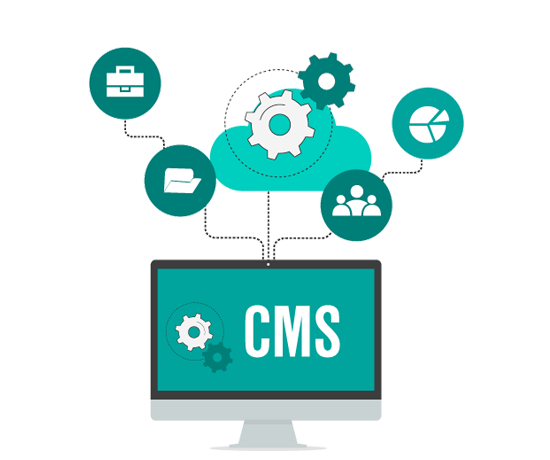
\includegraphics[width=1\textwidth]{img/cmsheader.png}
   \end{center}
\end{titlepage}


% Title page
\thispagestyle{empty}

\section*{Contactgegevens}

\begin{itemize}
	\item[]\textbf{Student}\ 
	\begin{itemize}
		\item[]{\makebox[5cm][l]{Naam} \StudentName}
		\item[]{\makebox[5cm][l]{Studentnummer} \StudentNumber}
		\item[]{\makebox[5cm][l]{Academisch jaar} \AcedemicYear}
		\item[]{\makebox[5cm][l]{E-mail} \StudentEmail}
		\item[]{\makebox[5cm][l]{Telefoonnummer} \StudentPhone}
	\end{itemize}

	\item[]
	
	\item[]\textbf{Onderwijsinstelling}\ 
	\begin{itemize}
		\item[]{\makebox[5cm][l]{Naam} NHL Stenden University of Applied Sciences}
		\item[]{\makebox[5cm][l]{Course} HBO-ICT}
		\item[]{\makebox[5cm][l]{Locatie} Rengerslaan 8-10, 8917 DD, Leeuwarden}
		\item[]{\makebox[5cm][l]{Telefoonnummer} +31 (0)88 991 7000}
	\end{itemize}

	\item[]
	
	\item[]\textbf{Docentbegeleider}\ 
	\begin{itemize}
		\item[]{\makebox[5cm][l]{Naam} \LecturerName}
		\item[]{\makebox[5cm][l]{Email} \LecturerEmail}
		\item[]{\makebox[5cm][l]{Telefoonnummer} \LecturePhone}
	\end{itemize}

	\item[]

	\item[]\textbf{Afstudeercommissie}\ 
	\begin{itemize}
		\item[]{\makebox[5cm][l]{Email} afstuderenschoolofict@nhlstenden.com}
	\end{itemize}
	
	\item[]

	\item[]\textbf{Examencommissie}\ 
	\begin{itemize}
		\item[]{\makebox[5cm][l]{Email} examencommissiehboict@nhlstenden.com}
	\end{itemize}

	\item[]
	
	\item[]\textbf{Organisatie}\ 
	\begin{itemize}
		\item[]{\makebox[5cm][l]{Naam} \OrganisationName}
		\item[]{\makebox[5cm][l]{Locatie} \OrganisationLocation}
		\item[]{\makebox[5cm][l]{Telefoonnummer} \OrganisationPhone}
	\end{itemize}

	\item[]
	
	\item[]\textbf{Bedrijfsbegeleider}\ 
	\begin{itemize}
        \item[]{\makebox[5cm][l]{Naam}Thom Koenders} 
		\item[]{\makebox[5cm][l]{Email} thom@snakeware.com}
		\item[]{\makebox[5cm][l]{Telefoonnummer} +31 (0)6 13 09 18 51}
		\item[]{\makebox[5cm][l]{Rol} Senior software developer }
	\end{itemize}

	\item[]

\end{itemize}

\newpage

\section*{Versiebeheer}
\begin{tabularx}{\textwidth}{|l|l|X|}
	\hline
	\textbf{Versie} & \textbf{Datum} & \textbf{Veranderingen} \\
	\hline
	1.0 & 6 oktober & Eerste versie \\  
    \hline
\end{tabularx}



% List of tables
% \listoftables
% \addcontentsline{toc}{chapter}{Lijst van tabellen}

% Glossary
\printnoidxglossaries
\addcontentsline{toc}{chapter}{Woordenlijst}

% table of contet 
\tableofcontents
% Content
% \newpage
% \cleardoublepage
\pagenumbering{arabic}
\setcounter{page}{1}
\chapter{Inleiding}
Dit is het technische verslag voor het \qw{Het CMS voor iedereen} project.
Het technische verslag is een onderdeel van de afstudeerperiode binnen NHL Stenden Hogeschool.
Het technische verslag dient als documentatie en verantwoording voor het product dat gemaakt is tijdens de afstudeerperiode.
In de volgende sectie wordt de organisatie beschreven verder wordt de aanleiding en de context van de afstudeeropdracht beschreven.

\section{Organisatieomschrijving}
Snakeware New Media B.V. (Snakeware) is een E-business bureau gevestigd in Sneek.
Haar aangeboden diensten omvatten het adviseren, bouwen en onderhouden van digitale
producties, met een focus op websites, webshops en mobiele apps \Parencite{SnakewareWhatWeDo}. Op
het moment van schrijven telt Snakeware meer dan 60 werknemers, elk met verschillende
specialiteiten. Ze leveren services aan organisaties zoals DPG Media, DekaMarkt
en Poiesz supermarkten \Parencite{SnakewareCases}.

\section{Context}
Snakeware heeft een platform genaamd \qw{Snakeware Cloud} dit platform is een \gls{CMS} waarmee ze digitale content kunnen voorzien voor haar (grotere) klanten.
Snakeware Cloud is een applicatie waarmee Snakeware en haar klanten webapplicaties kan inrichten en voorzien van content.

\whitespace[2]
De klant van Snakeware kan zijn of haar website zelf inrichten door middel van het specificeren van de content op de verschillende pagina’s.
Dit wordt gedaan door middel van artikelen die door het \gls{CMS} gebruikt kunnen worden.
De content van het artikel kan verschillen tussen simpele tekst, vragenlijst, webshop producten, etc.
Hiernaast zijn er ook \gls{SEO} opties binnen Snakeware Cloud om de site goed te kunnen vinden op het internet.
Hierbij zijn er opties zoals de mogelijkheid om de title tags en zoekwoorden toe te kunnen voegen in de head \Parencite{HTMLhead}

\whitespace[2]
Hierom heeft Snakeware Cloud veel features en configuratie stappen wat het complex en duur maakt om een relatief kleine webapplicatie te maken voor kleinere klanten.
Dit zorgt ervoor dat Snakeware zich niet kan vestigen in een markt met veel kleinere klanten, en hierdoor omzet misloopt.
 
\section{Aanleiding}
Het huidige platform is 21 jaar oud en er is veel functionaliteit in de loop der jaren aan toegevoegd.
Omdat Snakeware Cloud een oud platform is zijn er veel technieken en best practices gebruikt die nu niet meer als optimaal worden beschouwd.
Deze technieken waren erg geïntegreerd in Snakeware Cloud en er is in het verleden gekozen om niet de code te herschrijven om het aan de huidige standaarden te voldoen van andere projecten.
Een voorbeeld hiervan is het plaatsen van afkortingen voor de tabelnaam als prefix bij elke kolom, of gigantische C\# \Parencite{CSharp} files van 10 000 regels met verschillende functies.
Deze functies houden zich niet aan de \textit{Single Responsibility Principle} van de SOLID ontwerpmethode \Parencite{SOLID} wat het moeilijk maakt om het huidige \gls{CMS} te onderhouden.

\whitespace
Ook zijn er technieken toegepast die nu niet meer relevant zijn.
Een voorbeeld hiervan is dat het \gls{CMS} gebruikmaakt van JavaScript \Parencite{JavaScript} en toen ze er mee begonnen bestonden JavaScript classes \Parencite{JavascriptClasses} nog niet, dus hebben ze die zelf geïmplementeerd.
Deze oudere technieken en standaarden zorgen ervoor dat het meer tijd kost om het CMS te onderhouden vanwege de extra code.
Dit zorgt ervoor dat het meer tijd en geld kost om het Snakeware Cloud uit te breiden.
% \todo[inline]{ik wou graag bloat gebruiken inplaats van extra code maar volgens kan dat niet suggesities}
% Deze oudere technieken zorgen voor veel overhead en zorgt ervoor dat het veel tijd en geld kost om het \gls{CMS} uit te breiden.

\whitespace[2]
Een van de voornaamste uitdaging met Snakeware Cloud betreft de verouderde datastructuur van de applicatie.
Deze veroudering is het gevolg van een initïele ontwikkeling waarbij onvoldoende rekening werd gehouden met toekomstige functionaliteitsuitbreidingen in het systeem.
Als gevolg daarvan is de onderliggende datastructuur niet aangepast, maar zijn er elementen aan toegevoegd.
Dit heeft geresulteerd in database query's van duizenden regels en complexe relaties tussen tabellen in de database.
Dit huidige scenario bemoeilijkt aanzienlijk het toevoegen van nieuwe functionaliteiten, wat resulteert in aanzienlijke tijd en kosten investeringen.

\whitespace
Hierom wil Snakeware een nieuw systeem met een nieuwe datastructuur.
% Hierom wil Snakeware dat er een nieuwe datastructuur komt met de daar bij behoorende \gls{CMS}-API.
Door het gebruiken van een nieuwe softwarearchitectuur zouden er velen problemen opgelost kunnen worden die nu voor komen.
Omdat er een nieuwe datastructuur moet komen en de logica van het oude systeem nauw verbonden is met de datastructuur is het niet mogelijk om de oude code opnieuw te gebruiken.

\newpage
\section{Opdrachtomschrijving}
\label{sec:Opdrachtomschrijving}
De opdracht is om een proof of concept CMS-API te ontwikkelen die gebruikt maakt van een datamodel en systeemarchitectuur dat flexibeler, onderhoudbaarder is en gebruik maakt van moderne best practices.
Tijdens de afstudeeropdracht wordt er primair op het datamodel en de systeemarchitectuur gefocust.
Omdat er nog geen concreet datamodel en systeemarchitectuur is zal dit onderzocht en ontworpen moeten worden.

\whitespace[2]
De opdracht omvat het achterhalen van de requirements, ontwerpen en ontwikkelen van het proof of concept met als focus een nieuw datamodel, met de essentiële functionaliteiten.

\whitespace[2]
Het huidige Snakeware Cloud platform bestaat uit 2 verschillende \gls{GUI}:
\begin{itemize}
	\item[-] Snakeware Cloud \gls{GUI}
    \item[-] De \gls{Eindgebruiker} zijn webapplicatie
\end{itemize}

\whitespace
Met de Snakeware Cloud \gls{GUI} kan de \gls{Beheerder} de content van de website aanpassen.
Door middel van de webapplicatie van de \gls{Beheerder} kan de \gls{Eindgebruiker} de content bekijken en er mee interacteren.
Er is voor gekozen om niet de Snakeware Cloud \gls{GUI} te realiseren om de afstudeeropdracht in scope te houden.
Er is wel voor gekozen om de \gls{Beheerder} zijn webapplicatie in zijn minimale vorm uit te werken.
% Om de userflows van de afstudeeropdracht toch te kunnen testen wordt er gebruik gemaakt van postman workflows \Parencite{PostmanWorkflows}
% \todo[inline]{kijken of dit nog relevant is, als hier voor nog tijd voor is dan zal ik het implementren maar anders haal ik dit stukje weg}

\whitespace[2]
% Om de \gls{UserJourneys} te testen wordt er gebruikgemaakt van postman workflows \Parencite{PostmanWorkflows}.
Het doel van het proof of concept is dat er aangetoond kan worden dat door het gebruiken van een nieuw datamodel en systeemarchitectuur ook services verleend kunnen worden aan kleinere klanten.
Dit zou eventueel ook een startpunt zijn om op verder te bouwen.
% \todo[inline]{Feedback van justin: \textit{Deze paragraaf is nu niet gepast voor een onderzoeksverslag}}
% \todo[inline]{Misschien een stukje theoretisch kader/ voor onderzoek te hebben waarin je het CMS ietwat toelicht (misscien met plaatje wow) (De pre, zonder je deelvragen te beantwoorden). Ik weet alleen niet of ik hier genoeg tijd voor heb}
%

\section{Leeswijzer}
Het ontwerp wordt behandeld in hoofdstuk 2, hier wordt het datamodel toegelicht en de gebruikte softwarearchitectuur wordt behandeld.
In hoofdstuk 3 wordt de realisatie van het product besproken.
Hier wordt besproken hoe het eindproduct is gerealiseerd is en welke bouwmiddelen gebruikt zijn.
Daarna wordt in hoofdstuk 4 het beheer, validatie en verificatie van het product besproken.
Hier gaat het onder andere hoe de code kwaliteit is bewaakt en hoe de testen zijn uitgevoerd.
In hoofdstuk 5 wordt de conclusie en de aanbevelingen besproken.
En in het laatste hoofdstuk wordt er gereflecteerd op de afstudeerperiode en de verschillende competenties.


\include{Content/2_Onderzoeksopzet/Onderzoeksopzet}
\chapter{Resultaten}
Dit hoofdstuk omvat de deel 2 en 3 van de onderzoekscyclus beschreven in \textit{Wat is Onderzoek?} (zie figuur \ref{fig:VerzamelEnAnalyseerCyclusen}).
Dit wordt gedaan door de vragen te beantwoorden van hoofdstuk \ref{chap:Onderzoeksopzet}.
Dit hoofdstuk is opgedeeld in de verschillende deelvragen waarbij in elk hoofdstuk een andere deelvraag wordt besproken.

\begin{graphic}
	\vspace{0.2cm}
	\captionsetup{type=figure}
    \caption{Deel 2 en 3 van de onderzoekscylcus afgeleid van \textit{Wat is Onderzoek?}}
    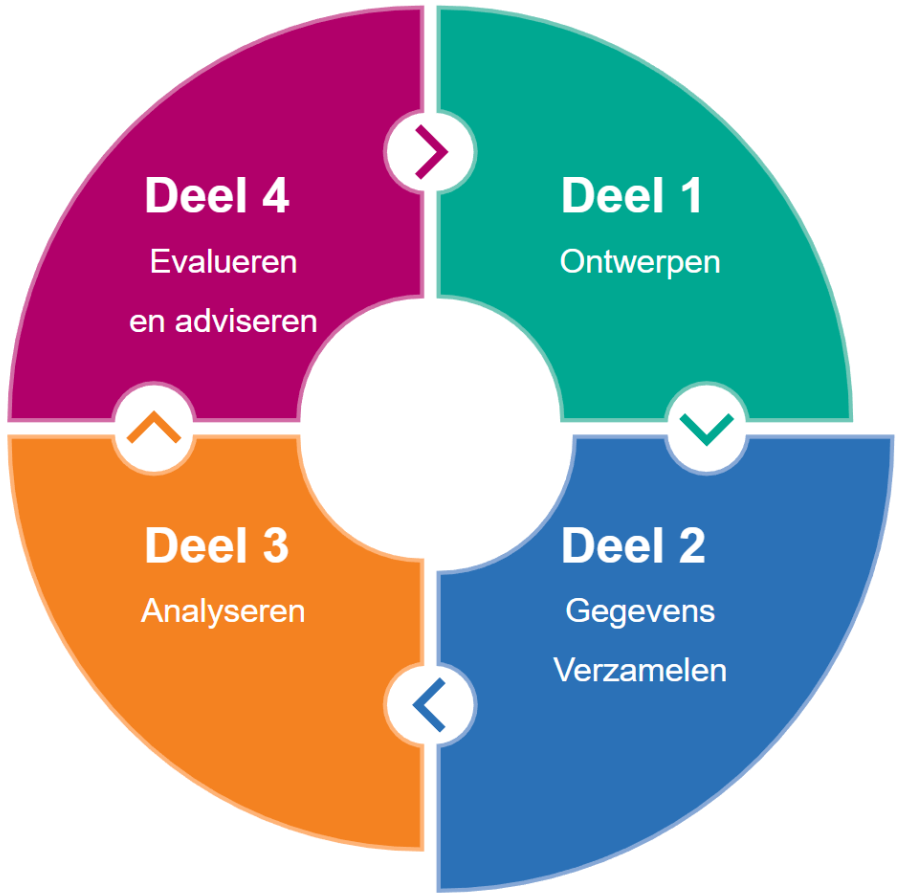
\includegraphics[scale=0.4]{img/GegevensVerzamelenCyclus.png}
	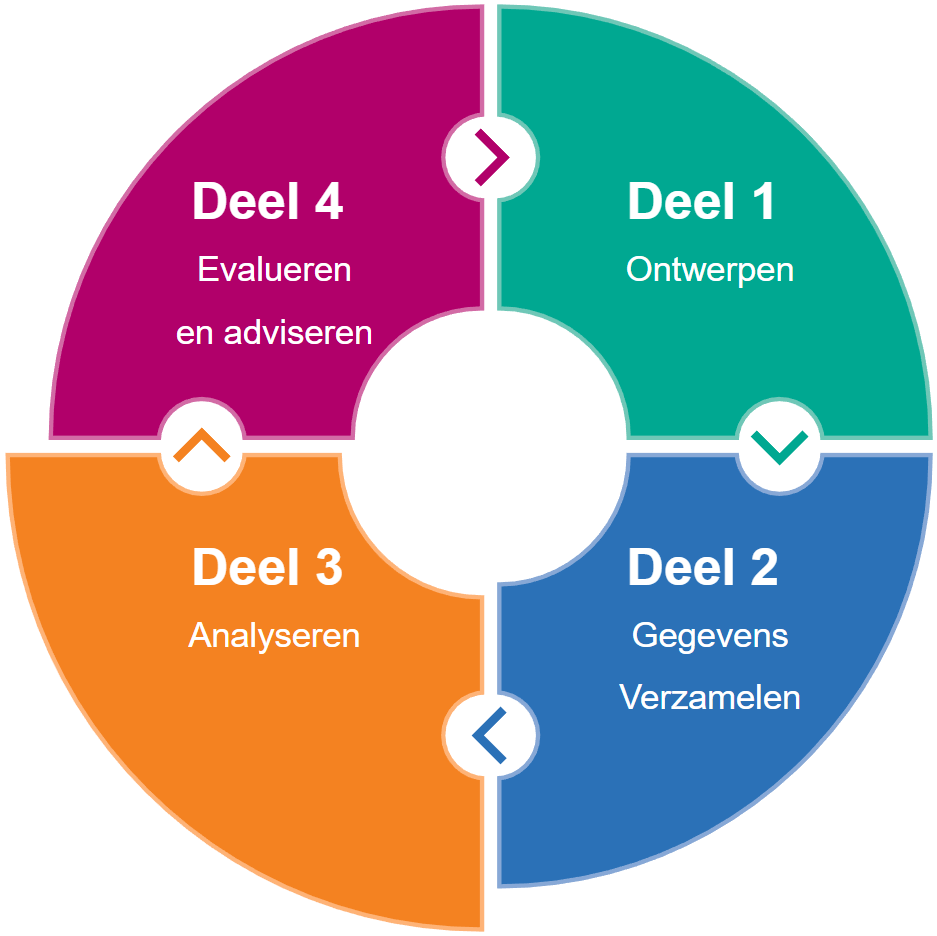
\includegraphics[scale=0.4]{img/AnalyserenCyclus.png}
		\label{fig:VerzamelEnAnalyseerCyclusen}
	\vspace{0.2cm}
\end{graphic}

\section{Deelvraag 1: Stakeholders}
De stakeholders zijn individuen of organisaties die invloed of belang hebben bij het project.
De product owner zal de mogelijke markt van kleine klanten representeren.
Dit wordt gedaan omdat Snakeware niet kleine klanten heeft die gebruikt kunnen worden als stakeholders.
% Sommige externe stakeholders zullen gerepresenteerd worden door een gekwalificeerde interne medewerker van Snakeware.
% Dit wordt gedaan omdat de afstudeeropdracht een proof of concept is, en de klanten van Snakeware hier nog niet bij betrokken worden.
Als na de afstudeerperiode het een succes blijkt te zijn en Snakeware wilt het verder ontwikkelen dan wordt contact opgezocht met de externe stakeholders (potentiële kleinere klanten). 
Er is een invloed matrix gemaakt (figuur \ref{fig:StakeholdersInvloedMatrix}) om de invloed en belang van de stakeholders te visualiseren. 
Het project bestaat uit de volgende stakeholders:

\whitespace
\textbf{Hans Hoomans (CEO):}
Hans Hoomans is een van de oprichters van Snakeware en is verantwoordelijk (samen met de andere directieleden) voor de toekomstvisie van Snakeware.
Tijdens het opstellen van de opdracht is al aangegeven dat Hans veel ideeën heeft voor een nieuw \gls{CMS} als een product onder Snakeware.
Hierom is besloten om hem mee te nemen in het project om de toekomstvisie te integreren in het project.

\whitespace
\textbf{Product Owner:}
De Product Owner is verantwoordelijk voor het vertegenwoordigen van de belangen, eisen en wensen van de kleinere klanten.
Deze kleinere klanten worden niet als individuele stakeholders beschouwd, aangezien Snakeware geen afzonderlijke kleine klanten heeft.
Om deze reden wordt er binnen Snakeware een gekwalificeerde persoon ingezet om hen te vertegenwoordigen.

\whitespace
\textbf{Afdeling R\&D:} De afdeling R\&D van Snakeware zijn de ontwikkelaars van het huidige \gls{CMS} en kunnen veel inzicht bieden in de huidige situatie / problemen.
Tijdens de realisatie en ontwerpfase kan er advies gevraagd worden aan de backend en frontend developers van het R\&D team.
Na de afstudeerperiode wordt het project overgedragen aan het R\&D team.
%
% \whitespace
% Het product bestaat uit twee software-applicaties een frontend die de data weergeeft aan de gebruiker, en een \gls{CMS}-API die de data serveerd voor de frontend.
% Deze twee software-applicaties worden na de afstudeerperiode overgedragen aan twee verschillende diseplines in Snakeware, namelijk de backend en frontend developers.
%
% \whitespace
% \textbf{Backend developers:} De \gls{CMS}-API wordt aan het einde van de afstudeeropdracht overgedragen aan de backend developers van Snakeware.
% Tijdens de ontwerp en realisatie fase kan er voor advies gevraagd worden over hoe de \gls{CMS}-API het best ontworpen / gerealiseerd kan worden. \\
% \textbf{Frontend developers} : De interface applicatie die gemaakt wordt om de data te tonen aan de gebruiker wordt ook overgedragen aan het einde van de afstudeeropdracht.
% Tijdens de ontwerp en realisatie fase kan er voor advies gevraagd worden over hoe de inteface het best ontworpen / gerealiseerd kan worden.

\whitespace
\begin{graphic}
    \captionsetup{type=figure}
    \caption{Stakeholders invloed matrix}
    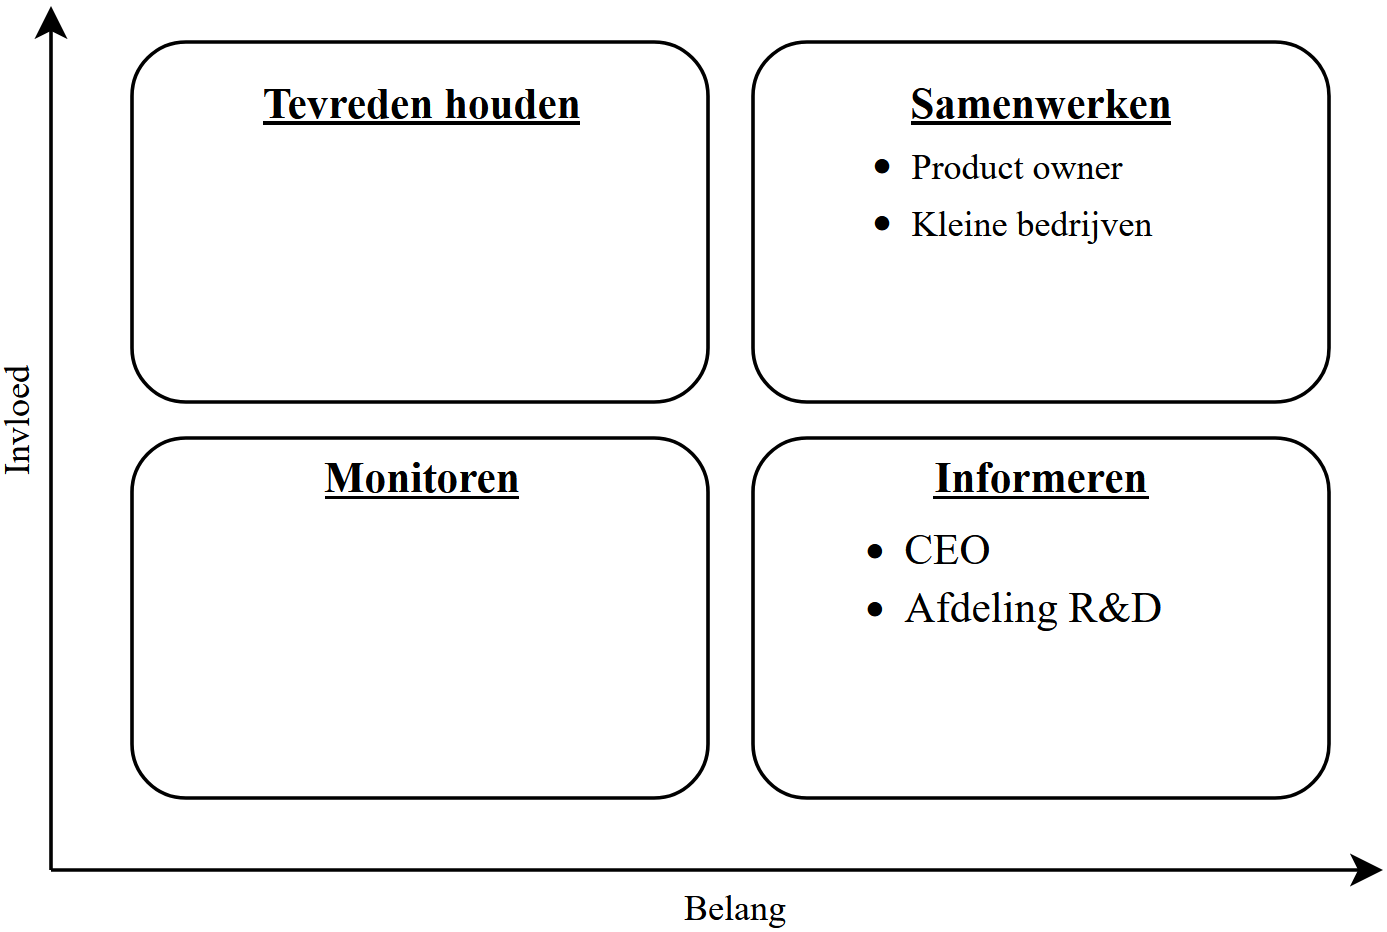
\includegraphics[scale=0.4]{StakeholdersInvloedMatrix}
    \label{fig:StakeholdersInvloedMatrix}
\end{graphic}

\todo[inline]{Het stakeholder verhaal uitzoeken na dat de herfst vakantie (voor of kleine klanten er we of niet er tussen moeten staan).}
\todo[inline]{De afbeelding klopt niet omdat hans er nog niet tussen staat en van wege het verhaal hier boven ik pas deze afbeelding aan als er bekend is wat er moet gebeuren met het verhaal hier boven.}
% \todo[inline]{Als er woorden over zijn maak een kleine samenvatting voor het resultaat}

\section{Deelvraag 2: Architectuur}
In deze paragraaf zijn de resultaten voor deelvraag 2 \textit{\SubquestionTwo} verzameld en onderzocht.
Er is samen met de architect van het CMS Erwin Keuning (ook wel de schepper genoemd) en met Software engineer Kevin Snijder een IT archtecture sketching sessie gedaan.
Samen met Erwin en Kevin is het huidige systeem architectuur en data model besproken en in beeld gebracht, de afbeeldingen die gebruikt worden zijn afgeleid van de originele tekening die te vinden is in BIJLAGE X.
Verder is ook gebruik gemaakt van internere documentatie van het CMS, om de tekingen te onderstuenen.
\todo[inline]{Voeg bijlage toe aan bestand}
\subsection{Het Systeem}
Het eerste gedeelte van het IT Architecuture sketching is besteed aan het globale systeem / flow van het systeem.
Er zijn op dit moment 3 verschillende Snakeware Cloud site methodes deze methodes zijn XSL, Vue 2 en Vue 3 site.
De Vue 2 en 3 werken door middel van de Snakware Cloud API en de XSL werkt door middel van de Snakeware.Site code base.
In afbeelding \ref{fig:SystemArchitectureXSL} is te zien hoe de XSL sites werken, in afbeeldingen \ref{fig:SystemArchitectureVue} is te zien hoe de vue sites werken. 

\whitespace
\begin{graphic}
	\captionsetup{type=figure}
	\caption{Globale systeem architectuur}
	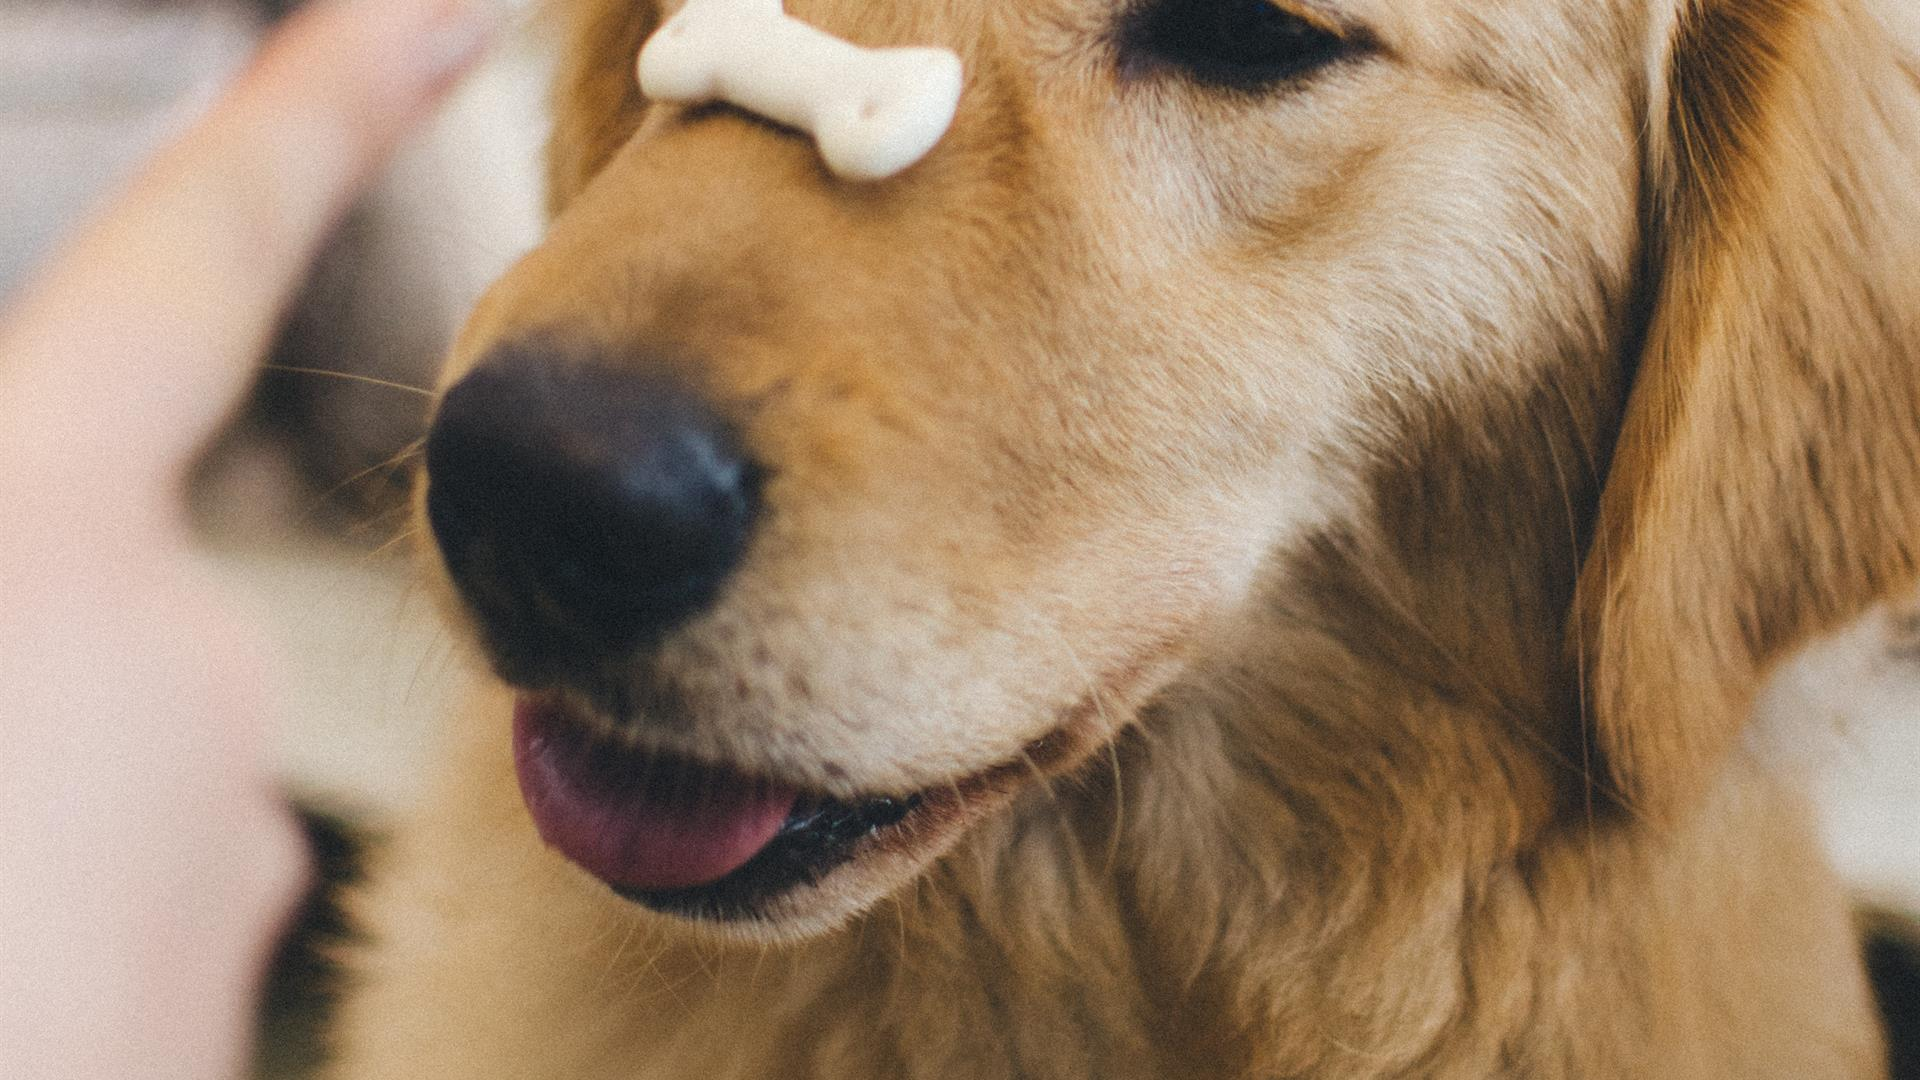
\includegraphics[scale=0.2]{Placeholder.jpg}
	\label{fig:SystemArchitectureXSL}
\end{graphic}

\whitespace
\begin{graphic}
    \captionsetup{type=figure}
    \caption{Globale systeem architectuur}
    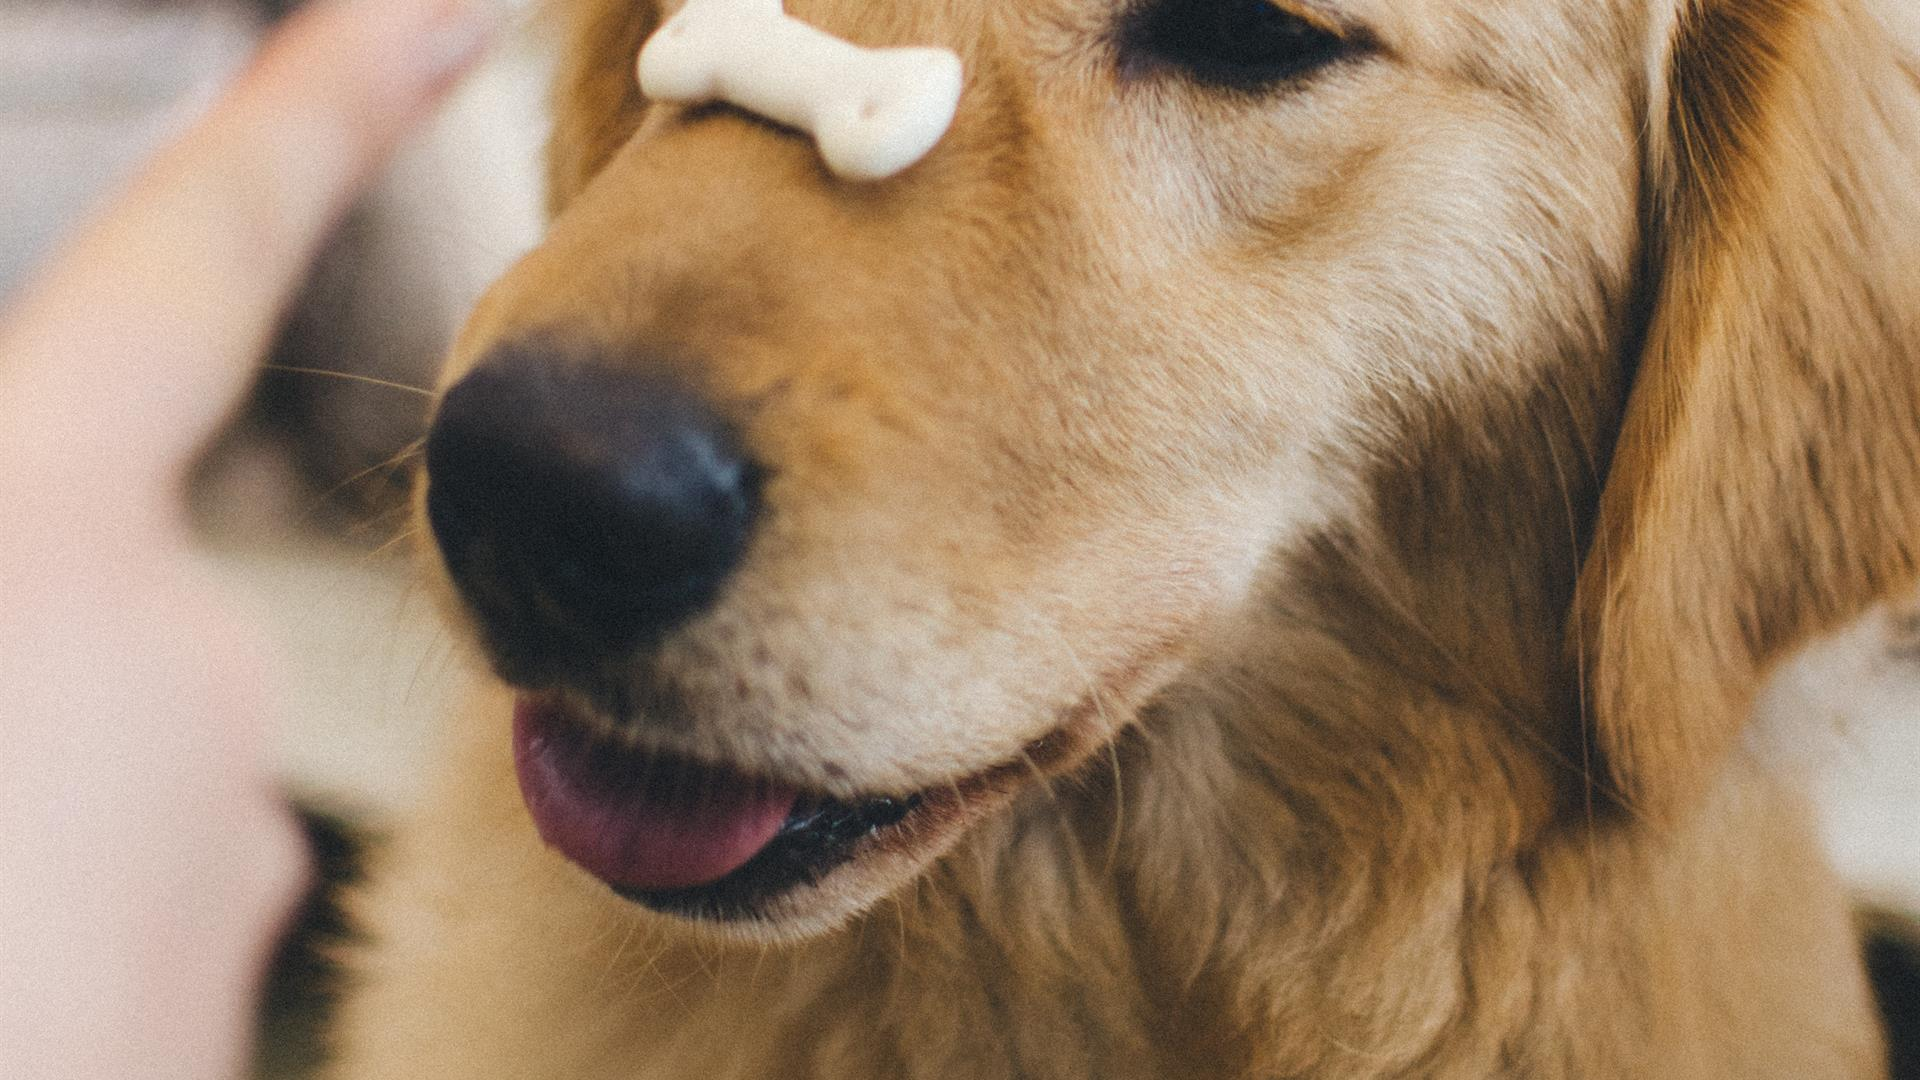
\includegraphics[scale=0.2]{Placeholder.jpg}
    \label{fig:SystemArchitectureVue}
\end{graphic}

Tijdens de IT Architeture sketching was er ook ruimte overgelaten om te onderzoeken waar er mogelijk verbeteringen gemaakt konden worden.
Een van de grote problemen nu met het huidige CMS is dat het niet gebruikt maakt van de SOLID prinicples (Personelijke cummunicatie erwin).
Ook is het CMS een grote Monolith dit zorgt er voor dat het niet goed schaalt met meerdere gebruikers.
Verder is het gebruik van XML ook niet optimaal meer dit is niet de snelste Data tranfer model en kan verbeterd worden.

\todo[inline]{Verbeter de teksten}
\todo[inline]{Opzoeken hoe je persoonlijke communicatie refereerd}

\subsection{Het Datamodel}
ook heel wow

\section{Deelvraag 3: Knelpunten}
In dit hoofdstuk worden resultaat van deelvraag 3 \qw{\textit{\SubquestionThree}} verzameld en geanalizeerd.
Voor deze deelvraag zijn er 2 expertinterviews gedaan met Janny Reitsma en Rob Douma.
Het interview met Janny is uitgevoerd op 31 oktober 2023 en het interview met Rob op 2 november 2023.
In de volgende hoofdstukken de belangrijkste punten van de interviews genoemd en behandeld.
De interviews zijn opgenomen en zijn transcripties van gemaakt die te vinden zijn in bijlage \ref{appendix:ExpertInterviews}

\subsection{Janny Reitsma interview}
\label{sec:JannyInterview}
Janny Reitsma werkt voor de service desk van Snakeware, en geeft cursussen aan nieuwe klanten die het CMS gaan gebruiken.
Verder handelt Janny ook vaak de vragen en functionaliteit aanvragen van klanten af voor het CMS.

\whitespace
Tijdens het interview kwam het naar voren dat Janny vindt dat \gls{SEO} erg belangrijk is voor het CMS en dat het nu nog niet optimaal wordt afgehandeld.
Klanten kunning het huidige CMS artikelen linken naar andere plekken op hun site.
Helaas komt het vaak voor dat klanten linken naar verkeerd pagina's waardoor ze vaak bij de service desk komen om dit op te lossen.
% Klanten kunnen op dit moment vaak fouten maken door verkeerd pagina's te linken aan elkaar waardoor het niet altijd goed gaat.
Verder moeten er voor sommige \gls{SEO} tools moeten er elementen in de applicatie geplaatst worden.
Bij deze elementen kun je denken aan zogenaamde Facebook pixel \Parencite{FacebookPixel}.
Verder moeten voor sommige \gls{SEO} opties elementen in de applicatie geplaatst worden.
Dit moet nu worden gedaan door een developer, dit kost tijd en geld hierdoor wordt Snakeware een duurdere partij.

\whitespace
Dit probleem speelt zich nu ook voor bij het integreren van derde partijen integraties.
Bij deze integraties kun je denken aan een cadeaubon widget of een kalender planner.
Het liefst wilt Snakeware dat de klant dit zelf kan doen zodat Snakeware als goedkopere partij er uit komt.

\whitespace
Een andere groot punt is dat het huidige CMS interface niet meer van deze tijd is.
Het zou meer visueel moeten werken zodat klanten makkelijker kunnen zien waar hun content staat en hoe het getoond worden.

\subsection{Rob Douma interview}
\label{sec:RobInterview}
Rob Douma is een oud informatieanalist die in de loop der jaren naar een product owner rol binnen Snakeware veranderd.
Verder richt hij vaak CMS omgeving in voor de grote klanten van het CMS en richt hij ook soms de database in.

Tijdens het interview kwam het naar voren dat Rob redelijk tevreden is met de huidige functionaliteiten van het CMS. 
Hierbij werd vooral gesproken over de formulieren functionaliteit en de aanpasbaarheid van de artikelen.
Volgens Rob moet zulke functionaliteit blijven zodat de klant meer zelf kan doen.

\whitespace
Een van de problemen die Rob wel aankaartte, is dat het CMS nog te rigide voelt in hoe content geplaatst moet worden.
Rob zou graag een oplossing willen waar mee hij  de artikelen van de websites makkelijker kan beheren en groeperen.
Deze groepen zou hij graag weer kunnen gebruiken bij andere artikelen

% Hierdoor kost het soms meer tijd om content goed op de site te kunnen zetten.
% Een mogelijke oplossing hiervoor gaf Rob aan is het groeperen van content op basis van een container model.
% Waarbij je artikelen kan groeperen in een container en deze container kan injecteren in andere artikelen.
%
\newpage
\whitespace
Tijdens het interview is er ook gesproken over de huidige database structuur van het CMS.
Rob gaf aan dat er op dit moment veel legacy data in de database zit met alle gevolgen van dien.
Ook gaf Rob aan dat er veel logica in de database zit door middel van triggers en stored procedures, en dit is liever niet gewenst.

\subsection{Samenvatting en antwoord}
Er zijn twee interviewen gedaan met experts binnen Snakeware, deze experts waren Janny Reitsma en Rob Douma.
In het interview van Janny kwam naar voren dat een van de grote knelpunten is de huidige implementatie van \gls{SEO}.
Ook kwam er naar voren dat de klant meer zelf moet kunnen inrichten door middel van derde partijen integratie.

\whitespace
Bij het interview van Rob kwam naar voren dat de huidige knelpunten bij de flexibiliteit van het inrichten van content.
Rob gaf ook aan dat hij graag wil dat de flexibiliteit van artikeltypes en formulieren moet blijven.
Na dat de resultaten waren verzameld waren zijn de resultaten terug gelegd bij Janny en Rob.
Zij hebben de resultaten als juist beschouwd.

\section{Deelvraag 4: Requirements}
wow deelvraag 4

\section{Deelvraag 5: Prioritering}
\label{sec:Prioritering}
In dit hoofdstuk wordt de deelvraag beantwoord \textit{\SubquestionFive}
De requirement die uit deelvraag 4 zijn gekomen worden gecategoriseerd in 4 verschillende categorieën.
Deze categorieën zijn bepaald door middel van de MoSCoW methode \Parencite{MoSCoW}.
De MoSCoW methode bestaat uit de volgende onderdelen:

\whitespace
\textbf{Must have:} Dit zijn de kern functionaliteiten, zonder deze functionaliteiten zou het project niet bruikbaar zijn en niet als succes beschouwd worden.

\whitespace[1]
\textbf{Should have:} Dit zijn de functionaliteiten die niet essentieel zijn maar wel belangrijke functionaliteiten toevoegen in het systeem.

\whitespace[1]
\textbf{Could have:} Dit zijn de functionaliteiten die je graag zou willen hebben.
Ze zijn niet essentieel als er tijd over is in het project zou je deze functionaliteiten realiseren.

\whitespace[1]
\textbf{Won't have:} Dit zijn de functionaliteiten die je zou willen zien in een ander stadium van een project.
Of als er tijd over is en al de andere functionaliteiten zijn al geimplementeerd.
\whitespace[2]
Om de requirement te categoriseren in de categorieën van de MoSCoW methode wordt er een score aan de requirement toe gewezen.
Deze score wordt bepaald door middel van formule \ref{eq:PioritizationRequirementsFormula}.

\whitespace
\begin{equation}
	\label{eq:PioritizationRequirementsFormula}
	Score = TS + OS + (9 - duur)
\end{equation}

\whitespace
Formule \ref{eq:PioritizationRequirementsFormula} bestaat uit de volgende aspecten:
\begin{enumerate}
	\item[-] Tevredenheidsscore (TS) [1,2,\ldots,5]: Deze waarden wordt toegekend door de stakeholder met betrekking van de requirement.
	      De stakeholder geeft een waarde van 1 tot 5 van tevredenheid als het geimplementeerd wordt.
	      Hierbij is een 1 niet erg tevreden en 5 erg tevreden.
	\item[-] Ontevredenheidscore (OS) [1,2,\dots,5]: Deze waarden wordt toegekend door de stakeholder met betrekking van de requirement.
	      De stakeholder geeft een waarde van 1 tot van ontevredenheid als het niet geimplementeerd wordt.
	      Hierbij is een 1 niet erg onteverden en een 5 erg ontevreden.
	\item[-] Duur [1,2,3,5,8]: De duur representeert door een relatief getal om de geschatte tijd om de requirement te implementeren te representeren.
	      De waardes van de duur zijn een verkleinde selectie van Scrum poker \Parencite{ScrumPoker}.
	      Deze waardes worden geverifieerd door een senior developer zodat hier een correcte schatting van gemaakt kan worden.
\end{enumerate}

\whitespace
Het maximum wat doormiddel van deze formule behaald kan worden is 18 (5 + 5 + (9 - 1) = 18) en het minimum wat behaald kan worden is 3 (1 + 1 + (9 - 8) = 3).
Door het verschil van deze getalen te verdelen over 4 categorien krijg je de volgende getallen ranges:

\whitespace
\makebox[3cm][l]{Must have:} $ x \in \mathbb{R} : 14 \leq x \leq 18 $ \\
\makebox[3cm][l]{Should have:} $ x \in \mathbb{R} : 9 \leq x \leq 13 $ \\
\makebox[3cm][l]{Could have:} $ x \in \mathbb{R} :  5 \leq x \leq 8 $ \\
\makebox[3cm][l]{Won't have:} $ x \in \mathbb{R} : 3 \leq x \leq 4 $

\newpage
\whitespace
Het resultaat van formule \ref{eq:PioritizationRequirementsFormula} en de categorisatie met behulp van de MoSCoW methode is te zien in Tabel \ref{tab:RequirementPrioritization}. %\ref{}
De requirements zijn voorzien van een verwachte duur en acceptatiecriteria.
Een voorbeeld user story is te zien in tabel \ref{rq:res5Sample}.
Dit leidt tot 5 must have, 6 should have, 1 could have en 2 wont have requirements de volledige lijst met geprioriteerde requirements is te vinden in bijlage \ref{appendix:Requirements}.

\begin{graphic}
	\vspace{0.2cm}
	\captionsetup{type=table}
	\caption{gepriotiriseerde requirement}
	\begin{tabular}{ |p{3cm}||p{1cm}|p{1cm}|p{1.5cm}|p{1cm}|p{2.5cm}| }
		\hline
		\multicolumn{6}{|c|}{Requirement prioritizatie lijst}       \\
		\hline
		Requirement id & TS & OS & Duur      & Score & Prioritering \\
		\hline
		KB-FR1         & 5  & 5  & 9 - 5 = 4 & 14    & Must have    \\
		KB-FR2         & 5  & 5  & 9 - 5 = 4 & 14    & Must have    \\
		KB-FR3         & 4  & 1  & 9 - 3 = 6 & 11    & Should have  \\
		KB-FR4         & 3  & 1  & 9 - 2 = 7 & 11    & Should have  \\
		KB-FR5         & 4  & 3  & 9 - 3 = 6 & 13    & Should have  \\
		KB-FR6         & 5  & 5  & 9 - 5 = 4 & 14    & Must have    \\
		KB-FR7         & 3  & 2  & 9 - 5 = 4 & 9     & Should have  \\
		KB-FR8         & 5  & 5  & 9 - 3 = 6 & 16    & Must have    \\
		KB-FR9         & 3  & 2  & 9 - 3 = 6 & 11    & Should have  \\
		KB-FR10        & 2  & 1  & 9 - 5 = 4 & 7     & Could have   \\
		KB-FR11        & 4  & 2  & 9 - 3 = 6 & 12    & Should have  \\
		KB-FR12        & 5  & 5  & 9 - 5 = 4 & 14    & Must have    \\
		SW-FR13        & 5  & 5  & 9 - 3 = 6 & 16    & Must have    \\
		SW-FR14        & 1  & 1  & 9 - 8 = 1 & 3     & Wont have    \\
		SW-FR13        & 1  & 1  & 9 - 8 = 1 & 3     & Wont have    \\
		\hline
	\end{tabular}	\label{tab:RequirementPrioritization}
	\vspace{0.2cm}
\end{graphic}

\begin{table}[!ht]
	\caption{Requirement - KR-FR1}
	\label{rq:res5Sample}
	\begin{tabularx}{\textwidth}{|m{0.5cm}|l|m{2.0cm}|l|m{3.5cm}|l|}
		\hline
		\textbf{Id} & KB-FR1 & \textbf{Prioriteit} & Must have & \textbf{Verwachte duur} & 5                                                                                                         \\
		\hline
		\multicolumn{6}{|p{\dimexpr\linewidth-2\arrayrulewidth-2\tabcolsep}|}{\textbf{User Story}}                                                                                                   \\
		\hline
		\multicolumn{6}{|p{\dimexpr\linewidth-2\arrayrulewidth-2\tabcolsep}|}{Als klein bedrijf wil ik content kunnen plaatsen op mijn website, zodat ik mijn informatie kan delen op het internet.} \\
		\hline
		\hline
		\multicolumn{6}{|p{\dimexpr\linewidth-2\arrayrulewidth-2\tabcolsep}|}{\textbf{Acceptatiecriteria}}                                                                                           \\
		\hline
		\multicolumn{6}{|p{\dimexpr\linewidth-2\arrayrulewidth-2\tabcolsep}|}{
		\begin{itemize}
			\item{Als klein bedrijf moet ik een Content kunnen plaatsen op mijn site.}
			\item{Het moet mogelijk zijn om een artikel te plaatsen (een artikel is een stuk text met een titel).}
			\item{Het moet mogelijk zijn om een afbeelding te plaatsen.}
			\item{Het moet mogelijk zijn om een video te kunnen plaatsen.}
		\end{itemize}}                                                                                        \\
		\hline
	\end{tabularx}
\end{table}
 

% \chapter{Conclusie}
dit is de conclusie

% \chapter{Reflectie}
dit is de reflectie

\printbibliography

% %TC:ignore
\appendix
\begin{appendix}
    \chapter{IT architecture sketching resultaat foto}
\label{appendix:ITArchitectureSketch}
\begin{center}
	\begin{graphic}
		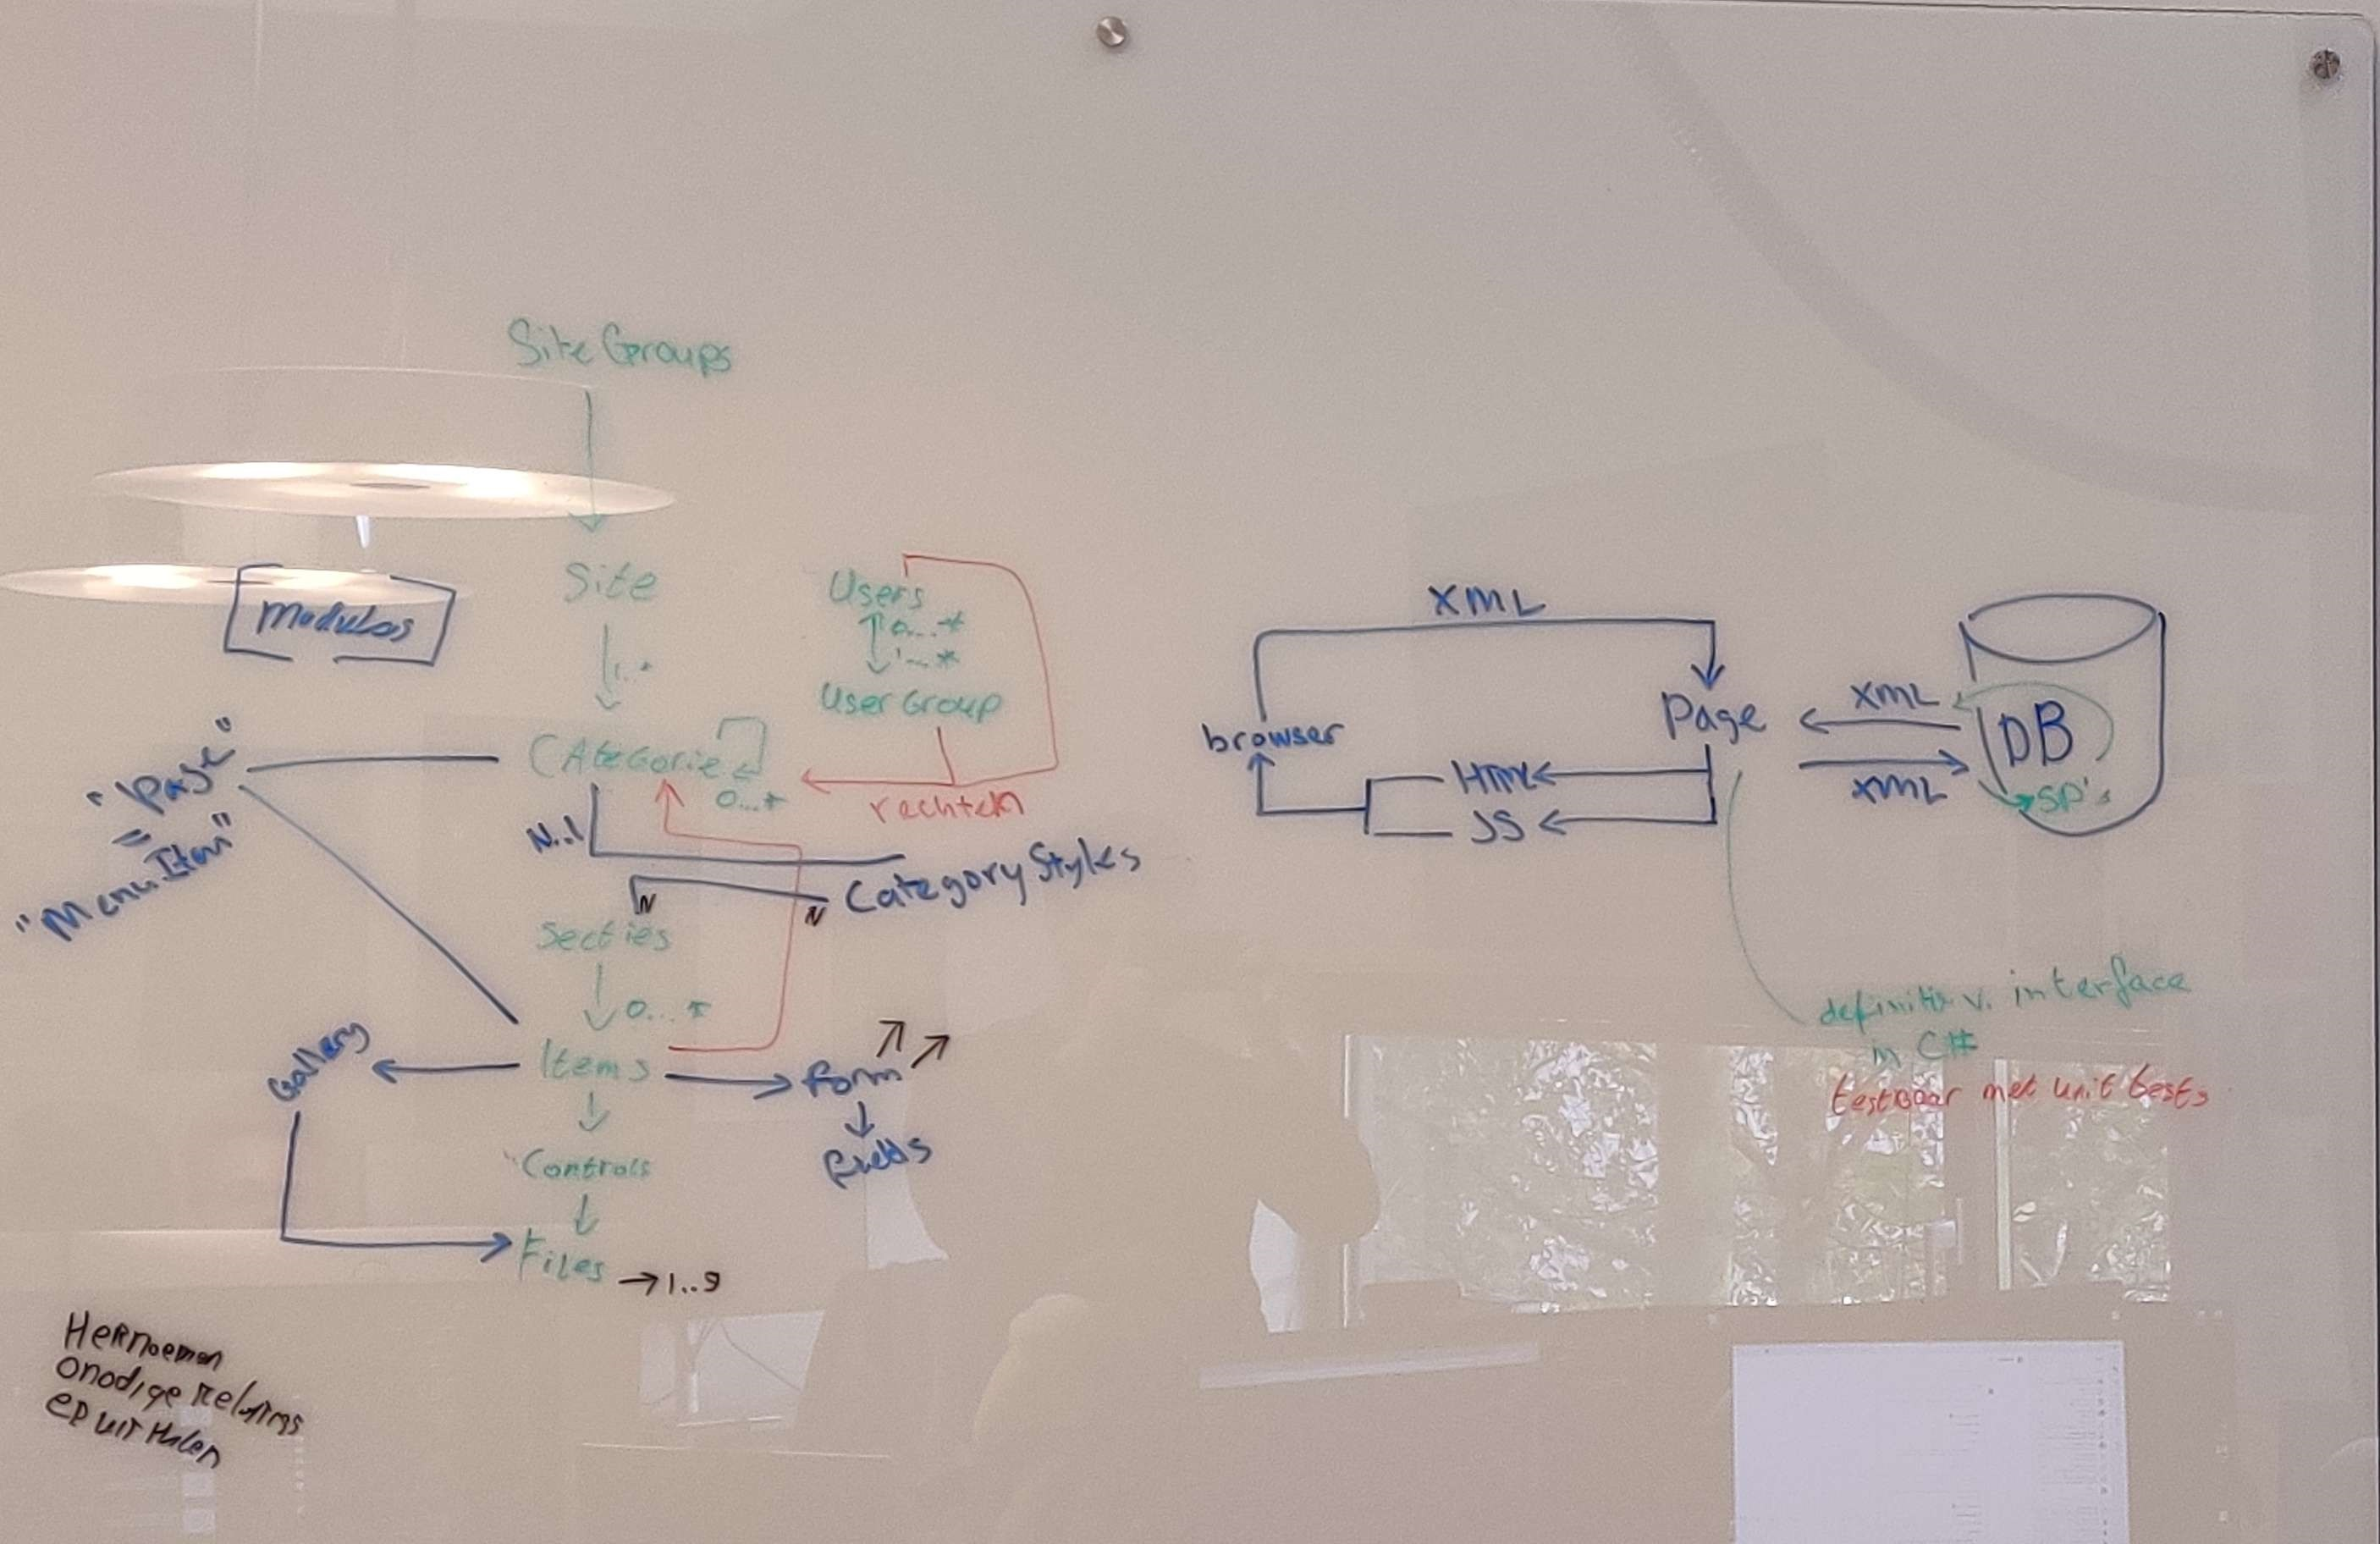
\includegraphics[scale=0.23]{ITArchitectureSketch}
	\end{graphic}
\end{center}


    \chapter{Expert Interviews}
\label{appendix:ExpertInterviews}
\todo[inline]{Transcribe interviews}
\section{Janny Reitsma Interview}
janny interview
\section{Rob Douma Interview}
rob interview

\end{appendix}

%TC:endignore
\end{document}
